\section{Results}
\label{sec:results}

\subsection{Encoder against decoder}

\Cref{tab:headline} and \cref{fig:headline} give the main comparison.
With the same data and training budget, every encoder recipe is above Qwen3-0.6B (\TestQwFull{}\% on the test set): \TestUbList{}\% with the softmax over ``yes'', and \TestUbYesNo{}\%, \TestUbSqrt{}\% and \TestUbSig{}\% with the softmax, the square-root softplus and the sigmoid over ``yes'' minus ``no''.
The encoder also has fewer parameters, 380M against 0.6B.
On the six external benchmarks the encoder recipes reach \ExtUbList{}\% to \ExtUbYesNo{}\%, against \ExtQwFull{}\% for the decoder.
The reproduced Qwen3-4B LoRA model, at \TestQwFourLora{}\%, remains ahead of all sub-billion models, so our claims are limited to models below one billion parameters.

\subsection{Full fine-tuning against LoRA}

The reproduced LoRA model of the same size reaches \TestQwLora{}\%, \DiffQwFullQwLoraAbs{} points below the fully fine-tuned decoder.
Both were trained on the same data, so this gap comes from updating all weights instead of a LoRA adapter, and accounts for about half of the \DiffUbSigQwLoraText{}-point gap between the best encoder recipe and the LoRA model.
The external accuracy of fully fine-tuned Qwen3-0.6B (\ExtQwFull{}\%) is not above that of its LoRA model (\ExtQwLora{}\%).

\subsection{Recipes}

Scoring by ``yes'' minus ``no'' gives most of the gain: over the ``yes'' logit alone it adds \DiffUbYesNoUbListAbs{} points on the test set and \ExtUbYesNo{}\% against \ExtUbList{}\% on the external benchmarks.
The sigmoid normalisation adds a further \DiffUbSigUbYesNoAbs{} points on the test set and nothing on the external benchmarks, and its results vary less between seeds.
The square-root softplus works like the sigmoid but has no upper bound, and it does no better than the softmax (\TestUbSqrt{}\% against \TestUbYesNo{}\%).
This suggests that the bound of the sigmoid is what helps.
The bound is not the only difference, though: for rejected options the square-root softplus also acts as a softmax at twice the temperature (\cref{sec:loss}).
\Cref{sec:analysis} compares the labels that each recipe predicts.

\subsection{How strongly the options depend on each other}
\label{sec:coupling}

In a softmax, raising one option's score lowers the probability of every other option, so the options are tied together.
DeepSeek-V3 gates its experts with a sigmoid instead \citep{deepseekv3}.
We test whether the normalisation changes how much the answer depends on the other options.
On the dev rows we shuffle the options four times and remove one wrong option, and count how often the answer changes (\cref{tab:coupling}).
Comparing the two softmax recipes shows the effect of the score; comparing the softmax and the sigmoid over ``yes'' minus ``no'' shows the effect of the normalisation.

The score does most of the work: ``yes'' minus ``no'' raises external accuracy from \CpExtYes{}\% to \CpExtYesNo{}\%, lowers the answer changes when a wrong option is removed from \CpDropYes{}\% to \CpDropYesNo{}\%, and lowers the largest gradient norm from \CpGradYes{} to \CpGradYesNo{}.
When the options are shuffled, the score and the sigmoid each lower the answer changes by about one point (\CpShufYes{}\%, \CpShufYesNo{}\%, \CpShufSig{}\%).
On top of the score, the sigmoid raises dev accuracy from \CpAccYesNo{}\% to \CpAccSig{}\%, lowers the calibration error from \CpEceYesNo{} to \CpEceSig{}, and brings the share of each predicted label closer to its share among the gold answers, which the score alone moves further away (total variation \CpLabelYes{}, \CpLabelYesNo{}, \CpLabelSig{}).
After training, the gold option's sigmoid averages only \CpSigGoldSig{}; far below 1, $\sigma(s)\approx e^{s}$, so the loss behaves almost like a softmax.
The square-root softplus has the smallest gradient spikes in training (largest norm \CpGradSqrt{}), but it changes its answer most often when the options are shuffled (\CpShufSqrt{}\%).

\subsection{Cost}

The encoder takes \MsUb{}\,ms per decision on one A100, one row at a time, against \MsQwFull{}\,ms for Qwen3-0.6B and \MsQwFourLora{}\,ms for Qwen3-4B.
\Cref{app:impl} gives the batched throughput.

\begin{table}[t]
  \centering\small
  \caption{Matched comparison: average accuracy (\%) over seeds. Test ALL is on the test set;
  Dev ALL and External are on the dev set and the six external benchmarks. Learning rates were chosen on
  dev. Bold: best below 1B parameters.}
  \label{tab:headline}
  % Generated by paper/figures/make_figures.py; do not edit.
\begin{tabular}{@{}llccc@{}}
\toprule
Model & Params & Dev ALL & Test ALL & External \\
\midrule
UltraBERT-380M, sigmoid\_norm & 380M & 72.7 & \textbf{72.1} & 59.5 \\
UltraBERT-380M, listwise & 380M & 71.2 & 69.7 & 57.8 \\
Qwen3-0.6B, full FT & 0.6B & 69.0 & 67.6 & 56.1 \\
Qwen3-0.6B, LoRA (released) & 0.6B & 64.5 & 63.0 & 56.9 \\
\midrule
Qwen3-4B, LoRA (released) & 4B & 79.3 & 77.3 & 73.5 \\
\bottomrule
\end{tabular}

\end{table}

\begin{figure}[t]
  \centering
  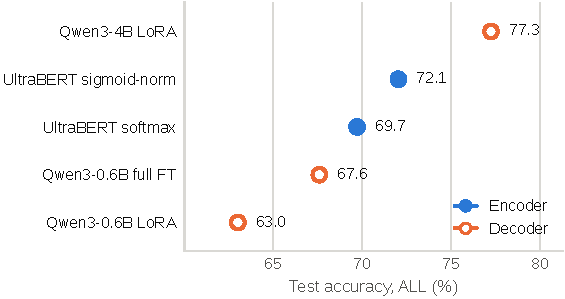
\includegraphics[width=0.62\linewidth]{fig_headline}
  \caption{Test accuracy (ALL, the mean over 13 datasets, on the test set, never used for any choice),
  averaged over seeds; \textcolor{encoder}{encoders} filled, \textcolor{decoder}{decoders} hollow.}
  \label{fig:headline}
\end{figure}

\begin{table}[t]
  \centering\small
  \caption{How strongly the options depend on each other, on the dev set (average scores). Each row is scored in four
  random option orders and once with one wrong option removed. TV: total variation between the predicted and the gold shares,
  over the three datasets with a fixed label set (label) and over option positions (position); lower is closer.
  Calibration error: expected calibration error of the top option's probability. $|s_k|$: size of the raw option scores. Bold: best in each row; accuracy is better higher, the other scores lower.}
  \label{tab:coupling}
  % Generated by paper/figures/make_figures.py; do not edit.
\begin{tabular}{@{}lccc@{}}
\toprule
& \begin{tabular}[b]{@{}c@{}}Softmax,\\``yes''\end{tabular} & \begin{tabular}[b]{@{}c@{}}Softmax,\\``yes'' $-$ ``no''\end{tabular} & \begin{tabular}[b]{@{}c@{}}Sigmoid-norm,\\``yes'' $-$ ``no''\end{tabular} \\
\midrule
Dev accuracy (\%) & 71.4 & 71.5 & \textbf{72.9} \\
\midrule
Answer changes, options shuffled (\%) & 15.6 & \textbf{12.7} & 13.7 \\
Answer changes, one wrong option removed (\%) & 5.9 & \textbf{4.3} & 4.9 \\
Largest gradient norm in training & 842 & 226 & \textbf{190} \\
\midrule
Label shares vs.\ gold (TV) & 0.167 & 0.219 & \textbf{0.139} \\
Position shares vs.\ gold (TV) & 0.050 & 0.048 & \textbf{0.041} \\
Calibration error, top option & 0.038 & 0.030 & \textbf{0.023} \\
Mean $|s_k|$ & 60.5 & 3.1 & 7.4 \\
\bottomrule
\end{tabular}

\end{table}
